\section{Auswertung}
\label{sec:Auswertung}
Alle Berechnungen werden mit dem Programm \glqq Numpy" \cite{numpy}, die Unsicherheiten mit dem Modul \glqq Uncertainties" \cite{uncertainties}, die Ausgleichsrechnungen mit dem Modul \glqq Scipy" \cite{scipy} durchgeführt und die grafischen Darstellungen über das Modul \glqq Matplotlib" \cite{matplotlib} erstellt.

\subsection{Spezifische Elektronenladung}

Die Messergebnisse des Durchgangs bei einer Beschleunigungsspannung von ${U_B=\SI{250}{\V}}$ sind in Tabelle \ref{tab:250} und die Messergebnisse bei eine Beschleunigungsspannung von ${U_B=\SI{380}{\V}}$ in Tabelle \ref{tab:380} aufgeführt. Jedes Kästchen hat eine Länge von ${s_K=\SI{6.25}{\milli\m}}$. Über 
\begin{equation}
    D=s_k\cdot A
\end{equation}
lässt sich die tatsächliche Strecke der Ablenkung $D$ bestimmen. 

\begin{table}
    \centering
    \caption{Abweichung des Elektronenstrahls in Abhängigkeit des an der Spule anliegenden Stroms bei einer Beschleunigungsspannung von $U_B=\SI{250}{\V}$}
    \begin{tabular}{S S S}
        \toprule
        {$I \:/\: \si{\ampere}$} & {$A \:/\:$ Kästchen} & {$D \:/\: \si{\centi\m}$}\\
        \midrule
        0.5 & 0.6 & 0.38  \\   
        1.0 & 1.0 & 0.63  \\
        1.5 & 1.4 & 0.88  \\
        2.0 & 1.8 & 1.13  \\
        2.5 & 2.2 & 1.38  \\
        \bottomrule
          
    \end{tabular}
    \label{tab:250}
\end{table}

\begin{table}
    \centering
    \caption{Abweichung des Elektronenstrahls in Abhängigkeit des an der Spule anliegenden Stroms bei einer Beschleunigungsspannung von $U_B=\SI{380}{\V}$}
    \begin{tabular}{S S S}
        \toprule
        {$I \:/\: \si{\ampere}$} & {$A \:/\:$ Kästchen} & {$D \:/\: \si{\centi\m}$} \\
        \midrule
        0.5 & 0.5  & 0.31 \\       
        1.0 & 0.75 & 0.47 \\
        1.5 & 1.1  & 0.69 \\
        2.0 & 1.5  & 0.94 \\
        2.5 & 1.75 & 1.09 \\ 
        \bottomrule
    \end{tabular}
    \label{tab:380}
\end{table}

In \eqref{eqn:V} lässt sich erkennen, dass der Ausdruck $\frac{D}{L^2 + D^2}$ über einen Proportionalitätsfaktor $a$ mit der magnetischen Feldstärke $B$ in Relation steht:
\begin{equation*}
    \frac{D}{L^2 + D^2} = \underbrace{\frac{1}{\sqrt{8U_B}} \sqrt{ \frac{e_0}{m_0}}}_{=a} B
\end{equation*}

Mit einem Wirkungsbereich $L=\SI{17.5}{\centi\m}$ lässt sich die Proportionalität zwischen $\frac{D}{L^2 + D^2}$ und der magnetischen Feldstärke in Abbildung \ref{fig:Kurve} grafisch darstellen. Der Proportionalitätsfaktor $a$ entspricht dabei der Steigung der durch die Werte gelegten Ausgleichsgerade. Da der Versuch mit zwei verschiedenen Beschleunigungsspannungen $U_B$ durchgeführt wird, sind in der Grafik \ref{fig:Kurve}, für den jeweiligen Messdurchlauf, zwei Ausgleichsgeraden abgebildet.
So ergeben sich die Geradenparameter der Ausgleichsgerade für den Versuchsdurchlauf bei einer Beschleunigungsspannung von $U_B=\SI{250}{\V}$ zu 
\begin{align*}
    a_1=&\SI{2539(4)}{\frac{1}{\tesla\meter}} \\
    b_1=&\SI{0.0418(0004)}{\frac{1}{\meter}}
\end{align*}
und bei einer Beschleunigungsspannung von $U_B=\SI{380}{\V}$ 
zu
\begin{align*}
    a_2=&\SI{2070(100)}{\frac{1}{\tesla\meter}} \\
    b_2=&\SI{0.030(010)}{\frac{1}{\meter}}.
\end{align*}

\begin{figure}
    \centering
    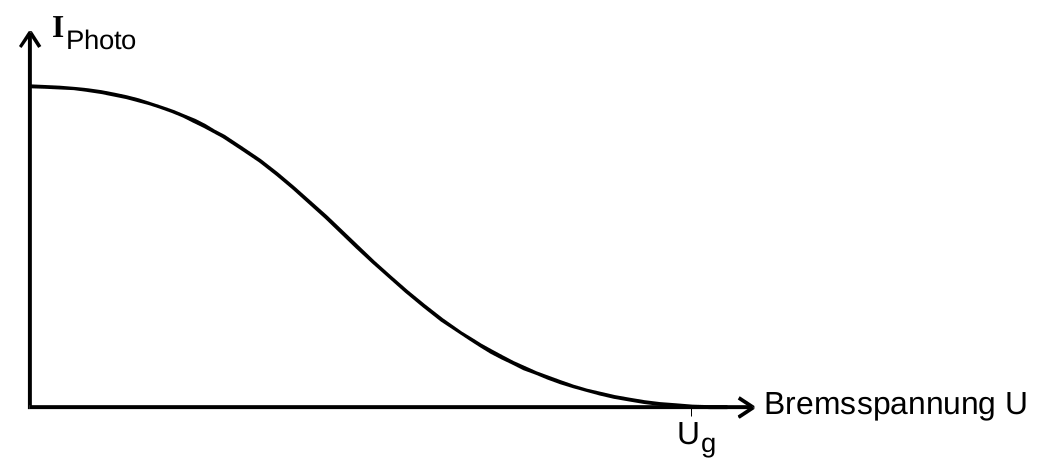
\includegraphics[width=\textwidth]{build/Kurve.pdf}
    \caption{B-Feld in Abhängigkeit des Verhältnisses zwischen den Strecken.}
    \label{fig:Kurve}
\end{figure}

Aus der Steigung der Ausgleichsgeraden
\begin{equation*}
    a=\frac{1}{\sqrt{8U_B}} \sqrt{ \frac{e_0}{m_0}}
\end{equation*}
lässt sich die spezifische Elektronenladung über
\begin{equation}
    \frac{e_0}{m_0}=8U_Ba^2
\end{equation}
bestimmen.
So lässt sich aus der Geradensteigung $a_1$ eine spezifische Elektronenladung von 
\begin{equation*}
    \frac{e_0}{m_0}=\SI{1.290(004)e10}{\coulomb\per\kilo\g}
\end{equation*} 
und aus der Geradensteigung $a_2$ eine spezifische Elektronenladung von
\begin{equation*}
    \frac{e_0}{m_0}=\SI{1.30(12)e10}{\coulomb\per\kilo\g}
\end{equation*}
bestimmen.
Werden diese beiden Werte gemittelt so lässt sich die spezifische Elektronenladung zu 
\begin{equation*}
    \frac{e_0}{m_0}=\SI{1.30(06)e10}{\coulomb\per\kilo\g}
\end{equation*} 
bestimmen.



\subsection{Totalintensität des Erdmagnetfeldes}
Die Horizontalkomponente des Erdmagnetfeldes lässt sich über den zur Kompensation benötigten Spulenstrom bestimmen. Dieser beträgt $I_{kom}= \SI{0.7}{\ampere}$ und ergibt über \ref{eqn:B} eine magnetisch Feldstärke von $B_{hor}=\SI{4.464e-05}{\tesla}$. Mit Kenntnis des Inklinationswinkel $\phi$, welcher im Versuch zu $\phi_{inkl}=\SI{58}{\degree}$ bestimmt wird, lässt sich über das Verhältnis
\begin{equation}
    B_{total}=\frac{B_{hor}}{\cos(\phi_{inkl})}
\end{equation} 
die Totalintensität des Erdmagnetfeldes zu $B_{total}=\SI{8.424e-05}{\tesla}$ bestimmen.



%Messwerte: Alle gemessenen physikalischen Größen sind übersichtlich darzustellen.
%
%Auswertung:
%Berechnung der geforderten Endergebnisse
%mit allen Zwischenrechnungen und Fehlerformeln, sodass die Rechnung nachvollziehbar ist.
%Eine kurze Erläuterung der Rechnungen (z.B. verwendete Programme)
%Graphische Darstellung der Ergebnisse